\documentclass[11pt]{article}
\usepackage[utf8]{inputenc}
\usepackage[russian]{babel}
\usepackage{amssymb}
\usepackage{amsmath}
\usepackage{graphicx}
\graphicspath{ {./images/} }

\let\oldemptyset\emptyset
\let\emptyset\varnothing

\begin{document}
	\begin{center}
	Вариант 7
	\end{center}
	
	\textit{\textbf{Задание 1}}

	\textit{Универсальное множество состоит из 26 строчных букв латинского
алфавита. Заданы множества A, B, C и D. Вычислить мощность множеств X
и Y.}

\textit{Даны множества
$A=\{b,f,g,m,o\}, B=\{b,g,h,l,u\}, C=\{e,f,m\}, D=\{e,g,l,p,q,u,v\}$\\
Вычислить мощность множеств}
$$X = (A \backslash C) \cup (B \cap C),
Y=(A \cap \bar B) \cup (D \backslash C) $$

\underline{Решение:}

1. Определим элементы множества 
$X = (A \backslash C) \cup (B \cap C)$.

Для этого найдём сначала разность множеств $A \backslash C$.
Для этого вычеркнем из множества $A=\{b,f,g,m,o\}$ элементы
$\{f, m\}$, принадлежащие $C=\{e,f,m\}$. Следовательно,
$A \backslash C = \{b, g, o\}$.
Затем найдём пересечение множеств $B \cap C$.
Множества $B$ и $C$ не имеют общих элементов. Следовательно,
$B \cap C = \emptyset$.
Таким образом, объединение $(A \backslash C) \cup (B \cap C)$ состоит из
трёх элементов $\{b, g, o\}$.

Мощность множества 
$X = (A \backslash C) \cup (B \cap C)$ равна 3.

2. Определим элементы множества 
$Y=(A \cap \bar B) \cup (D \backslash C)$

Найдем дополнение B . Универсальное множество по условию задания
состоит их 26 букв
$\{a,b,c,d,e,f,g,h,i,j,k,l,m,n,o,p,q,r,s,t,u,v,w,x,y,z\}$.
Если отсюда исключить 5 элементов множества $B$, то получим множество
$B$ из 21 элемента
$\{a,c,d,e,f,i,j,k,m,n,o,p,q,r,s,t,v,w,x,y,z\}$.

Пересечение множеств $A \cap \bar B$
состоит из элементов $\{f, m, o\}$, т.е. всех
элементов множества $A$, которые не принадлежат $\bar B$.

Для нахождения разности множеств $D \backslash C$ вычеркнем из множества
$D=\{e,g,l,p,q,u,v\}$
элемент $\{e\}$, принадлежащий
$C=\{e,f,m\}$. Получим
$D \backslash C = \{g, l, p, q, u, v\}$. В итоге\\
$$Y=(A \cap \bar B) \cup (D \backslash C) = \{f,g,l,m,o,p,q,u,v\}$$
Мощность множества Y равна 9. В данном случае множества $D \backslash C$
и $A \cap \bar B$ не пересекаются и мощность объединения равна
сумме мощностей слагаемых

Card Y=3+6

\pagebreak

\textit{\textbf{Задание 2}}

\textit{Задайте множество, указанное на рисунке с использованием
характеристического свойства множества:}

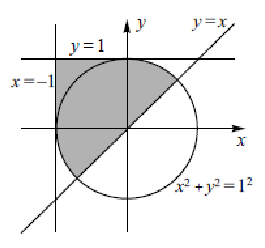
\includegraphics{task2}

\underline{Решение:}

Предлагаем вначале выразить это множество через системы и
совокупности:

$\left[ 
  \begin{gathered} 
    \left\{ 
      \begin{gathered} 
		  x^2 + y^2 \leq 1, \hfill 
        \\ 
        y \geq x \hfill 
        \\ 
      \end{gathered} 
    \right. \hfill 
    \\ 
    \left\{ 
      \begin{gathered} 
		  x^2+y^2 \geq 1, \hfill 
        \\ 
        y \geq 0, \hfill 
        \\ 
        y \leq 1, \hfill 
        \\ 
        x \leq 0, \hfill 
        \\ 
        x \geq -1, \hfill 
        \\ 
      \end{gathered} 
    \right. \hfill 
    \\ 
  \end{gathered} 
\right.$
\\[3pt]

Теперь запишем с использованием характеристического
свойства множества, используя для систем операцию пересечения
множеств, а для совокупности - объединения:

$$X=\{(x;y) \vert x^2+y^2 \leq 1, y \geq x\} \cup \{(x;y)\vert
x^2 + y^2 \geq 1, y \geq 0, y \leq 1, x \leq 0, x \geq -1\}$$


\end{document}
